\begin{boxK}{Conjoint-Measurement-Theory}
  Messaxomie fürs Intervallskalenniveau sind teilweise prüfbar über ein Conjoint-Measurement-Experiment. Hierbei geht man davon aus, dass $P=f(A,X)$ wobei $f$ eine non-interaktive Funktion ist. Geprüft werden muss die einfache Aufhebung (single cancellation) und die dopplete Aufhebung (double cancellation). Die einfache Aufhebung besagt, dass alle Zeilen und Spalten der Conjoint-Measurement-Matrix die gleiche Ordnung haben müssen. Die Doppelaufhebung restringiert die möglichen Ordnungen der Matrix. Wenn alle Spalten und Zeilen bereits geordnet sind, lässt sich über folgende Visualisierung die Doppelaufhebung prüfen. Hierbei entsprechen die Pfeile, dem $\leq$-Zeichen. Dünne Pfeile zwischen den Zellen repräsentieren die Antezedenz-Ordnungsbeziehungen, und dicke Pfeile repräsentieren die Konsequenz-Ordnungsbeziehung. 
  
\tikzset{
pics/alwaysthesame/.style={code={%

    % Draw the grid
    \draw[very thin, gray] (0, 0) grid (3, 3);
    
    % Add row labels
    \foreach \x in {1, 2, 3} {
        \node at (\x-0.5, 3.25) {$x_{\x}$};  % x1, x2, x3 labels
    }

    % Add column labels
    \foreach \y in {1, 2, 3} {
        \node at (-0.25, 3.5-\y) {$a_\y$};  % a1, a2, a3 labels
    }
    

    }
}}

% 1
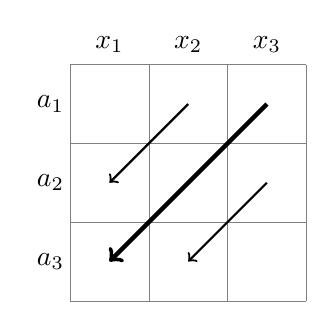
\begin{tikzpicture}
    \pic{alwaysthesame};
        % Draw error lines (arrows)
    \draw[->, thick] (1.5, 2.5) -- (0.5, 1.5);  % (1,2) to (2,1)
    \draw[->, ultra thick] (2.5, 2.5) -- (0.5, 0.5);  % (1,3) to (3,1)
    \draw[->, thick] (2.5, 1.5) -- (1.5, 0.5);  % (2,3) to (3,2)
\end{tikzpicture}
% 2
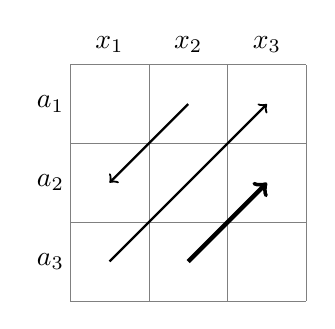
\begin{tikzpicture}
    \pic{alwaysthesame};
        % Draw error lines (arrows)
    \draw[->, thick] (1.5, 2.5) -- (0.5, 1.5);  % (1,2) to (2,1)
    \draw[->, thick] (.5, .5) -- (2.5, 2.5);  % (1,3) to (3,1)
    \draw[->, ultra thick] (1.5, 0.5) -- (2.5, 1.5);  % (2,3) to (3,2)
\end{tikzpicture}
% 3
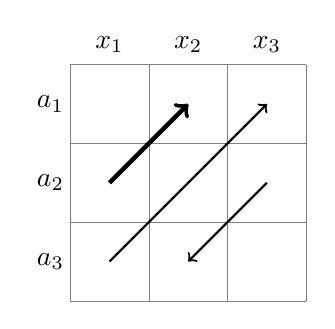
\begin{tikzpicture}
    \pic{alwaysthesame};
        % Draw error lines (arrows)
    \draw[->, ultra thick] (0.5, 1.5) -- (1.5, 2.5);  % (1,2) to (2,1)
    \draw[->, thick] (.5, .5) -- (2.5, 2.5);  % (1,3) to (3,1)
    \draw[->, thick] (2.5, 1.5) -- (1.5, 0.5);  % (2,3) to (3,2)
\end{tikzpicture}

% 4
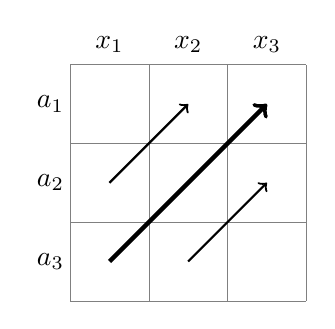
\begin{tikzpicture}
    \pic{alwaysthesame};
        % Draw error lines (arrows)
    \draw[->, thick] (0.5, 1.5) -- (1.5, 2.5);  % (1,2) to (2,1)
    \draw[->, ultra thick] (.5, .5) -- (2.5, 2.5);  % (1,3) to (3,1)
    \draw[->, thick] (1.5, 0.5) -- (2.5, 1.5);  % (2,3) to (3,2)
\end{tikzpicture}
%% 5
%
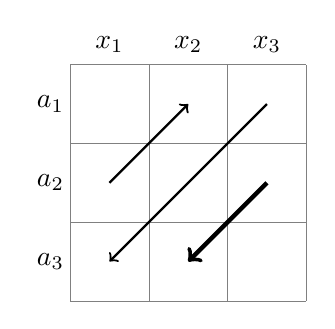
\begin{tikzpicture}
    \pic{alwaysthesame};
        % Draw error lines (arrows)
    \draw[->, thick] (0.5, 1.5) -- (1.5, 2.5);  % (1,2) to (2,1)
    \draw[->, thick] (2.5, 2.5) -- (0.5, 0.5);  % (1,3) to (3,1)
    \draw[->, ultra thick] (2.5, 1.5) -- (1.5, 0.5);  % (2,3) to (3,2)
\end{tikzpicture}
% 6
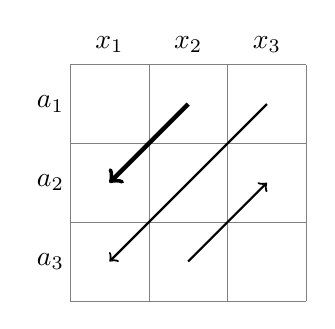
\begin{tikzpicture}
    \pic{alwaysthesame};
        % Draw error lines (arrows)
    \draw[->, ultra thick] (1.5, 2.5) -- (0.5, 1.5);  % (1,2) to (2,1)
    \draw[->, thick] (2.5, 2.5) -- (0.5, 0.5);  % (1,3) to (3,1)
    \draw[->, thick] (1.5, 0.5) -- (2.5, 1.5);  % (2,3) to (3,2)
\end{tikzpicture}
\end{boxK}
